%%%%%%%%%%%%%%%%%%%%%%%%%%%%%%%%%%%%%%%%%
% Short Sectioned Assignment LaTeX Template Version 1.0 (5/5/12)
% This template has been downloaded from: http://www.LaTeXTemplates.com
% Original author:  Frits Wenneker (http://www.howtotex.com)
% License: CC BY-NC-SA 3.0 (http://creativecommons.org/licenses/by-nc-sa/3.0/)
%%%%%%%%%%%%%%%%%%%%%%%%%%%%%%%%%%%%%%%%%

%----------------------------------------------------------------------------------------
%	PACKAGES AND OTHER DOCUMENT CONFIGURATIONS
%----------------------------------------------------------------------------------------

\documentclass[paper=a4, fontsize=11pt]{scrartcl} % A4 paper and 11pt font size

% ---- Entrada y salida de texto -----

\usepackage[T1]{fontenc} % Use 8-bit encoding that has 256 glyphs
\usepackage[utf8]{inputenc}
%\usepackage{fourier} % Use the Adobe Utopia font for the document - comment this line to return to the LaTeX default

% ---- Idioma --------

\usepackage[spanish, es-tabla]{babel} % Selecciona el español para palabras introducidas automáticamente, p.ej. "septiembre" en la fecha y especifica que se use la palabra Tabla en vez de Cuadro

% ---- Otros paquetes ----

\usepackage{url} % ,href} %para incluir URLs e hipervínculos dentro del texto (aunque hay que instalar href)
\usepackage{hyperref}
\hypersetup{
	colorlinks=true,
	linkcolor=black,
	urlcolor=black,
	citecolor=black,
}
\usepackage{amsmath,amsfonts,amsthm} % Math packages
%\usepackage{graphics,graphicx, floatrow} %para incluir imágenes y notas en las imágenes
\usepackage{graphics,graphicx, float} %para incluir imágenes y colocarlas

% Para hacer tablas comlejas
%\usepackage{multirow}
%\usepackage{threeparttable}

%\usepackage{sectsty} % Allows customizing section commands
%\allsectionsfont{\centering \normalfont\scshape} % Make all sections centered, the default font and small caps

\usepackage{fancyhdr} % Custom headers and footers
\pagestyle{fancyplain} % Makes all pages in the document conform to the custom headers and footers
\fancyhead{} % No page header - if you want one, create it in the same way as the footers below
\fancyfoot[L]{} % Empty left footer
\fancyfoot[C]{} % Empty center footer
\fancyfoot[R]{\thepage} % Page numbering for right footer
\renewcommand{\headrulewidth}{0pt} % Remove header underlines
\renewcommand{\footrulewidth}{0pt} % Remove footer underlines
\setlength{\headheight}{13.6pt} % Customize the height of the header

\numberwithin{equation}{section} % Number equations within sections (i.e. 1.1, 1.2, 2.1, 2.2 instead of 1, 2, 3, 4)
\numberwithin{figure}{section} % Number figures within sections (i.e. 1.1, 1.2, 2.1, 2.2 instead of 1, 2, 3, 4)
\numberwithin{table}{section} % Number tables within sections (i.e. 1.1, 1.2, 2.1, 2.2 instead of 1, 2, 3, 4)

\setlength\parindent{0pt} % Removes all indentation from paragraphs - comment this line for an assignment with lots of text

\newcommand{\horrule}[1]{\rule{\linewidth}{#1}} % Create horizontal rule command with 1 argument of height
\usepackage{booktabs}

\usepackage{listings}
\lstdefinelanguage
[x64]{Assembler}     % add a "x64" dialect of Assembler
[x86masm]{Assembler} % based on the "x86masm" dialect
{morekeywords={CDQE,CQO,CMPSQ,CMPXCHG16B,JRCXZ,LODSQ,MOVSXD, %
		POPFQ,PUSHFQ,SCASQ,STOSQ,IRETQ,RDTSCP,SWAPGS, %
		rax,rdx,rcx,rbx,rsi,rdi,rsp,rbp, %
		r8,r8d,r8w,r8b,r9,r9d,r9w,r9b, %
		r10,r10d,r10w,r10b,r11,r11d,r11w,r11b, %
		r12,r12d,r12w,r12b,r13,r13d,r13w,r13b, %
		r14,r14d,r14w,r14b,r15,r15d,r15w,r15b}} % etc.
\usepackage{color}
\usepackage{xcolor}
\lstdefinestyle{customc}{
	belowcaptionskip=1\baselineskip,
	breaklines=true,
	frame=L,
	xleftmargin=\parindent,
	language=C,
	showstringspaces=false,
	basicstyle=\footnotesize\ttfamily,
	keywordstyle=\bfseries\color{green!40!black},
	commentstyle=\itshape\color{purple!40!black},
	identifierstyle=\color{blue},
	stringstyle=\color{orange},
}

\lstset{escapechar=@,style=customc}
\usepackage{url}


\title{	
	\normalfont \normalsize
	\begin{figure}[htb]
		\centering
		
\includegraphics[width=0.3\textwidth]{./imagenes/1}
	\end{figure}
	\textsc{\textbf{Estructura de Computadores} \\ Grado en Ingeniería Informática \\ 
	Curso 2018-2019} \\ [25pt] % Your university, school and/or department name(s)
	\begin{figure}[htb]
		\centering
		
\includegraphics[width=0.15\textwidth]{./imagenes/2}
	\end{figure}
	\horrule{0.5pt} \\[0.4cm] % Thin top horizontal rule
	\huge Memoria Práctica 5. \\
	\huge E/S con Arduino.
	\\ % The assignment title
	\horrule{2pt} \\[0.5cm] % Thick bottom horizontal rule
}
\author{Félix Ramírez García  \\
\href{mailto:felixramirezgarcia@correo.ugr.es}{felixramirezgarcia@correo.ugr.es}} % Nombre y apellidos
\date{\normalsize\today} % Incluye la fecha actual

%----------------------------------------------------------------------------------------
% DOCUMENTO
%----------------------------------------------------------------------------------------

\begin{document}
	
	\maketitle % Muestra el Título
	
	\newpage %inserta un salto de página
	
	\tableofcontents % para generar el índice de contenidos
	
	\listoffigures % para generar índice de imágenes.
	
	\listoftables % para generar índice de tablas.
	
	\newpage
	
	%-----------------------------------------------------------------------
	%				   			Introduccion
	%-----------------------------------------------------------------------
	\section[Introduccion]{Introduccion}
	
	A continuación se van a mostrar varios ejemplos de uso de Elegoo , se mostrara para cada caso su código final,
	un esquema , una imagen y un breve vídeo con el programa funcionando. \\
	
	Para descargar y ver los vídeos se proporciona un enlace a Consigna UGR, se ha subido el archivo con la durabilidad máxima
	posible, que es de un mes. Si para la corrección de la practica hubiese expirado este tiempo, póngase en contacto conmigo por el correo indicado 
	en la primera pagina y le facilitaré un enlace actualizado . El enlace es el siguiente: \\
	
	\href{https://consigna.ugr.es/f/97a9Z8BMzWkM7KLa/videos.rar}{Para descargar vídeos pinchar aquí.}
	
	%-----------------------------------------------------------------------
	%				   Hacer parpadear el led de la placa
	%-----------------------------------------------------------------------
	\section[Hacer parpadear el led de la placa]{Hacer parpadear el led de la placa}
	
	El código que se ha cargado en la placa Elegoo para hacer parpadear la luz led de la placa ha sido el siguiente: 
	
	\lstset{language=C}
	\begin{lstlisting}[frame=single]
void setup(){
	pinMode(LED_BUILTIN, OUTPUT);
}

void loop(){
	digitalWrite(LED_BUILTIN, HIGH);
	delay(1000);
	digitalWrite(LED_BUILTIN, LOW);
	delay(1000);
}
	\end{lstlisting}
	
	En este caso el esquema eléctrico no es necesario, ya que simplemente se ha conectado la placa al ordenador por USB.\\
	
	El vídeo correspondiente a este caso se encuentra en la carpeta comprimida dentro de Consigna (Enlace en la introducción),
	su nombre es led\_placa.mp4
	
	%-----------------------------------------------------------------------
	%					Led de placa parpadea a mas velocidad
	%-----------------------------------------------------------------------
	\section[Zumbador pasivo]{5.1 Zumbador pasivo}
	
	El código que se ha cargado en la placa Elegoo para hacer un zumbador pasivo ha sido el siguiente: 
	
	\lstset{language=C}
	\begin{lstlisting}[frame=single]
#include "pitches.h"

// notes in the melody:
int melody[]={NOTE_D4,NOTE_E4,NOTE_E4,NOTE_F4,NOTE_D4,NOTE_E4,NOTE_E4,NOTE_F4,NOTE_C4,
			  NOTE_D4,NOTE_F4,NOTE_G4,NOTE_C4,NOTE_D4,NOTE_F4,NOTE_G4,NOTE_B4,NOTE_A4};

int noteDurations[] = {4,4,4,4,4,4,4,4,4,4,4,4,4,4,4,4,4,4};

void setup() {

}

void loop() {
	// iterate over the notes of the melody:
	for (int thisNote = 0; thisNote < 18; thisNote++) {
		// to calculate the note duration, take one second divided by the note type.
		//e.g. quarter note = 1000 / 4, eighth note = 1000/8, etc.
		int noteDuration = 1000 / noteDurations[thisNote];
		tone(8, melody[thisNote], noteDuration);

	// to distinguish the notes, set a minimum time between them.
	// the note's duration + 30% seems to work well:
int pauseBetweenNotes = noteDuration * 1.30;
delay(pauseBetweenNotes);
// stop the tone playing:
noTone(8);
}
}
	\end{lstlisting}
	
	El esquema eléctrico para hacer un zumbador pasivo es el que muestra la imagen 3.1. \\
	
	\begin{figure}[htb]
		\centering
		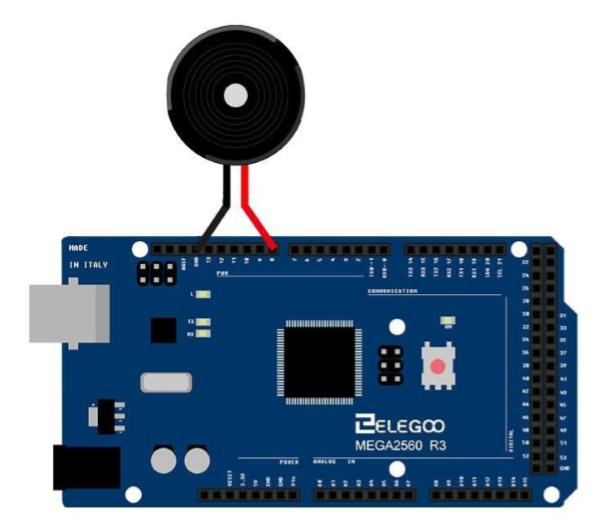
\includegraphics[width=0.7\textwidth]{./imagenes/3}
		\caption{Esquema zumbador pasivo} \label{fig:1}
	\end{figure}
	
	El vídeo correspondiente a este caso se encuentra en la carpeta comprimida dentro de Consigna (Enlace en la introducción),
	su nombre es zumbador\_pasivo.mp4 . 
	
	%-----------------------------------------------------------------------
	%					Led de placa parpadea a mas velocidad
	%-----------------------------------------------------------------------
	\section[Theremín de luz]{Theremín de luz}
	
	El código que se ha cargado en la placa Elegoo para hacer un Theremin de luz ha sido el siguiente: 
	
	\lstset{language=C}
	\begin{lstlisting}[frame=single]
// variable to hold sensor value
int sensorValue;
// variable to calibrate low value
int sensorLow = 1023;
// variable to calibrate high value
int sensorHigh = 0;
// LED pin
const int ledPin = 13;

void setup() {
	// Make the LED pin an output and turn it on
	pinMode(ledPin, OUTPUT);
	digitalWrite(ledPin, HIGH);

	// calibrate for the first five seconds after program runs
	while (millis() < 5000) {
		// record the maximum sensor value
		sensorValue = analogRead(A0);
		if (sensorValue > sensorHigh) {
			sensorHigh = sensorValue;
		}
		// record the minimum sensor value
		if (sensorValue < sensorLow) {
			sensorLow = sensorValue;
		}
	}

	// turn the LED off, signaling the end of the calibration period
	digitalWrite(ledPin, LOW);
}

void loop() {
	//read the input from A0 and store it in a variable
	sensorValue = analogRead(A0);

	// map the sensor values to a wide range of pitches
	int pitch = map(sensorValue, sensorLow, sensorHigh, 50, 4000);

	// play the tone for 20 ms on pin 8
	tone(8, pitch, 20);

	// wait for a moment
	delay(10);
}	
	\end{lstlisting}
	
	El esquema eléctrico para hacer un un Theremin de luz es el que muestra la imagen 4.1 :
	
	\begin{figure}[htb]
		\centering
		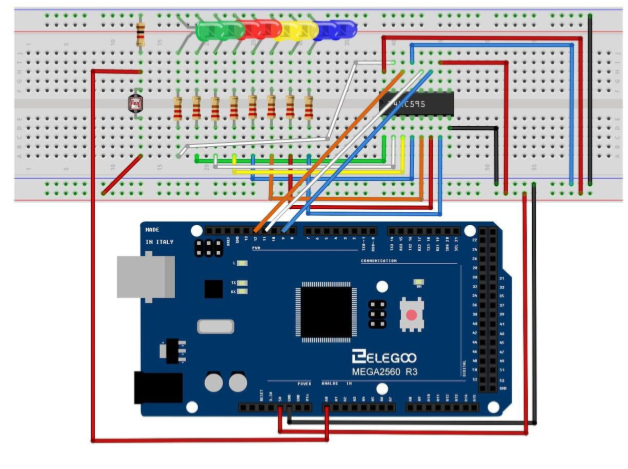
\includegraphics[width=0.7\textwidth]{./imagenes/4}
		\caption{Esquema Theremin de luz} \label{fig:1}
	\end{figure}
	
	Y la figura 4.2 muestra una imagen con la instalación realizada en el laboratorio. \\
	
	\begin{figure}[htb]
		\centering
		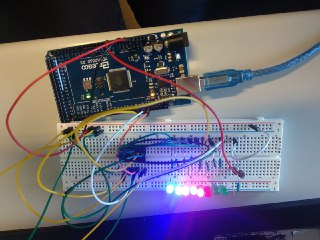
\includegraphics[width=0.7\textwidth]{./imagenes/5}
		\caption{Montaje Theremin de luz en laboratirio} \label{fig:1}
	\end{figure}
	
	El vídeo correspondiente a este caso se encuentra en la carpeta comprimida dentro de Consigna (Enlace en la introducción),
	su nombre es theremin\_luz.mp4
		
	%-----------------------------------------------------------------------
	%							BIBLIOGRAFIA
	%-----------------------------------------------------------------------
	% Referencia a bibliografia			En \cite{Baz}
	% Referencia a figura				La figura (\ref{fig:1})
	% Espacio entre lineas				\vspace{0.06in}
	% Figura con comentario al pie
	%\begin{figure}[htb]
	%	\centering
	%	
\includegraphics[width=0.4\textwidth]{./imagenes/1}
	%	\caption{Universidad de Granada.} \label{fig:1}
	%\end{figure}
	%\begin{thebibliography}{99}
	%	\bibitem{Baz} 
	%	\textsc{Bazaraa, M.S., J.J. Jarvis}
	%	\textit{Programacuib}.
	%	\newline
	%	\url{https://www.google.es}	
	%\end{thebibliography}

	


\end{document}